\documentclass{article}
\usepackage[margin=1.5cm]{geometry}
\usepackage{tikz}
\usepackage{amsmath}
\begin{document}

\section*{Konstruksi Segitiga dengan Sisi 5, 6, dan 7}

Kode lengkap gambar yang dibahas di artikel: membangun segitiga $ABC$
dengan $a = BC = 5$, $b = AC = 6$, dan $c = AB = 7$ menggunakan dua
busur jangka (dalam TikZ: lingkaran putus-putus berjari-jari 5 dan 6
yang berpotongan di titik $C$).

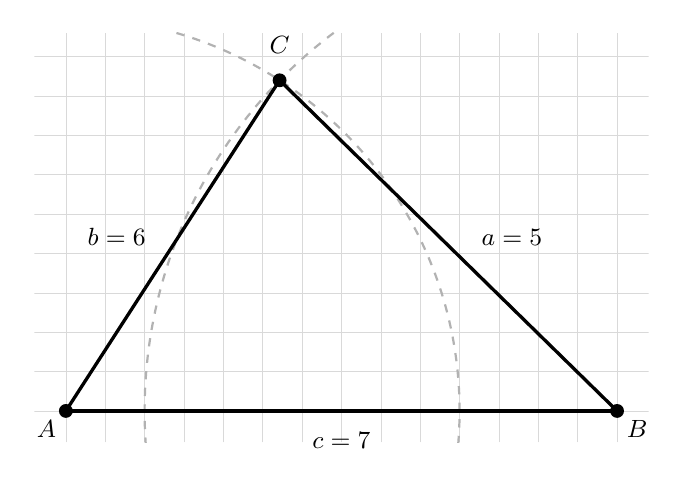
\begin{tikzpicture}[scale=1.0]
  \coordinate (A) at (0,0);
  \coordinate (B) at (7,0);
  % |AC|=5, |BC|=6  ->  x = (b^2 - a^2 + c^2)/(2c) = 38/14, y = sqrt(25 - x^2)
  \coordinate (C) at (2.7143,4.1991);
  \begin{scope}
    \clip (-0.4,-0.4) rectangle (7.4,4.8);
    \draw[gray!30, very thin] (-0.4,-0.4) grid[step=0.5] (7.4,4.8);
    \draw[dashed, gray!60, thick] (A) circle (5);   % busur jangka dari A, jari-jari b = 6? lihat catatan
    \draw[dashed, gray!60, thick] (B) circle (6);
  \end{scope}
  \draw[very thick] (A) -- (B) node[midway, below=4pt, font=\small] {$c=7$};
  \draw[very thick] (A) -- (C) node[pos=0.45, above left=2pt, font=\small] {$b=6$};
  \draw[very thick] (B) -- (C) node[pos=0.45, above right=2pt, font=\small] {$a=5$};
  \fill (A) circle (2.5pt) node[below left, font=\small] {$A$};
  \fill (B) circle (2.5pt) node[below right, font=\small] {$B$};
  \fill (C) circle (2.5pt) node[above=6pt, font=\small] {$C$};
\end{tikzpicture}

\bigskip
Catatan: busur dari $A$ berjari-jari $AC = 6$, busur dari $B$
berjari-jari $BC = 5$; keduanya berpotongan di $C$ (dan di bayangan
$C$ pada sebelah bawah garis $AB$).

\end{document}
